% Human activity -> Environment -> Welfare cycle
% (alternative to human_environment_welfare.svg; not referenced by lecture12.qmd)
\documentclass[tikz,border=4pt]{standalone}
\renewcommand\familydefault{\sfdefault}
\usetikzlibrary{arrows.meta}
\begin{document}
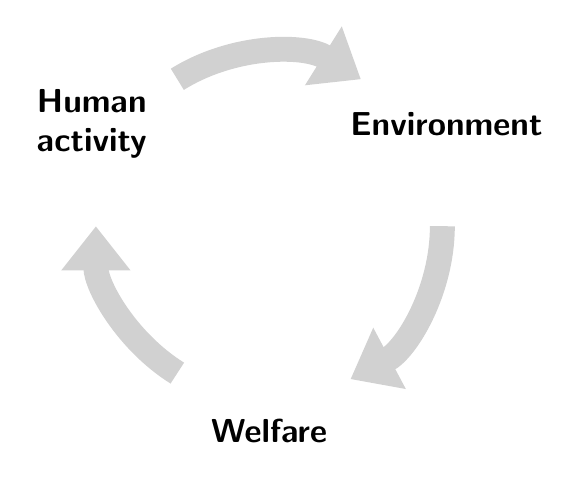
\begin{tikzpicture}[
    lbl/.style={font=\bfseries\large, align=center},
    cyc/.style={line width=9pt, draw=black!18, -{Triangle[length=16pt,width=24pt]}}
  ]
  \def\R{2.2}   % radius of the arrow ring
  \def\L{2.6}   % radius of the labels
  \node[lbl] at (150:\L) {Human\\activity};
  \node[lbl] at (30:\L)  {Environment};
  \node[lbl] at (270:\L) {Welfare};
  \draw[cyc] (122:\R) arc[start angle=122, end angle=58,  radius=\R];
  \draw[cyc] (0:\R)   arc[start angle=0,   end angle=-62, radius=\R];
  \draw[cyc] (238:\R) arc[start angle=238, end angle=180, radius=\R];
\end{tikzpicture}
\end{document}
